\chapter{Solved Examples}
\thispagestyle{empty}
\label{chap11}

\section{Solved Examples}

%---------------RC circuit-------------------
\subsection{Basic RC Circuit}
\subsubsection{Problem Statement:} Plot the Input and Output Waveform of an RC circuit whose input voltage (Vs) is 50Hz, 3V peak to peak. The values of Resistor (R) and Capacitor(C) are $1k$ and $1uf$ respectively.
\subsubsection{Solution:}
\begin{itemize}
\item Creating a Project:
The new project is created by clicking the {\tt New} icon on the menubar. The name of the project is given in the pop up window as shown in \figref{rc1}.
\begin{figure}[!htp]
    \centering
    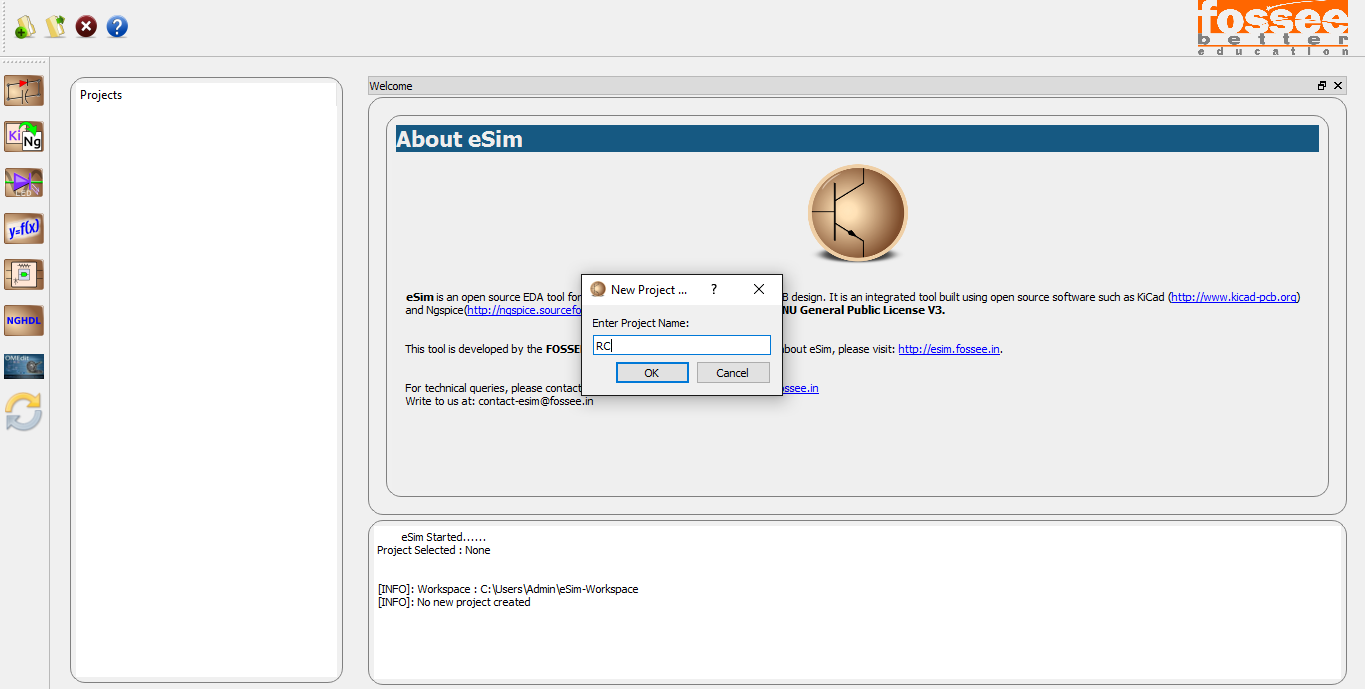
\includegraphics[width=\hgfig]{figures/rc1.png}
    %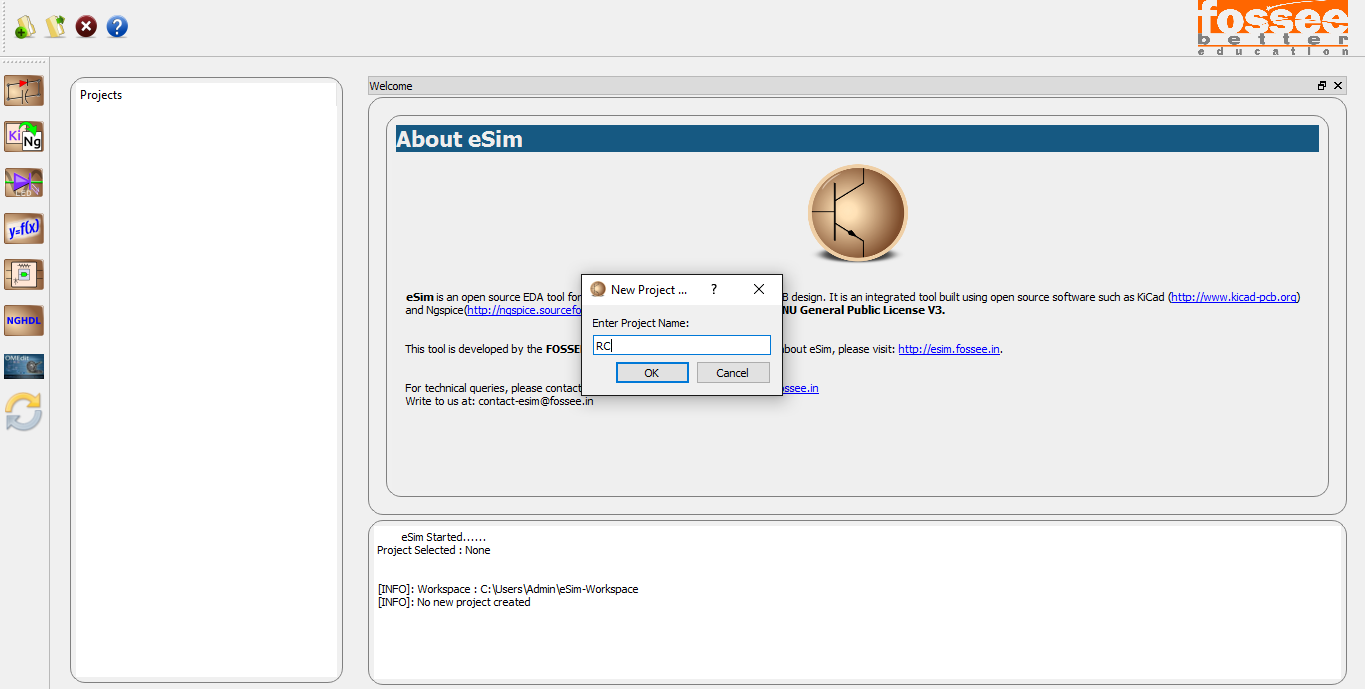
\includegraphics[width=\linewidth]{figures/rc1.png}
    \caption{Creating New Project}
    \label{rc1}
\end{figure}

\item Creating the Schematic:
To create the schematic, click the very first icon of the left toolbar as shown in the \figref{rc2}. This will open KiCad Eeschema.

\begin{figure}[!htp]
    \centering
    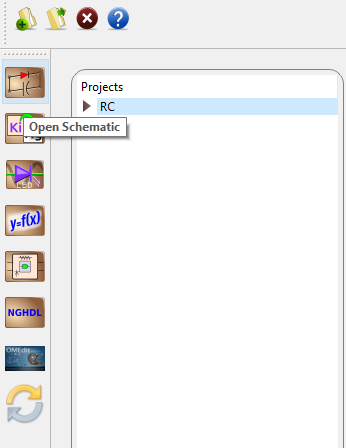
\includegraphics[width=\smfigp]{figures/rc2.png}
    %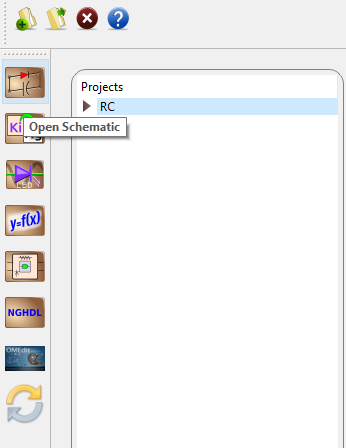
\includegraphics[width=\linewidth]{figures/rc2.png}
    \caption{Open Schematic Editor}
    \label{rc2}
\end{figure}

To create a schematic in KiCad, we need to place the required components. \figref{rc_component} shows the icon on the right toolbar which opens the component library.

\begin{figure}[!htp]
    \centering
    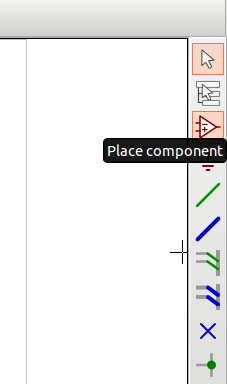
\includegraphics[width=\tnfig]{figures/rc_component.png}
    %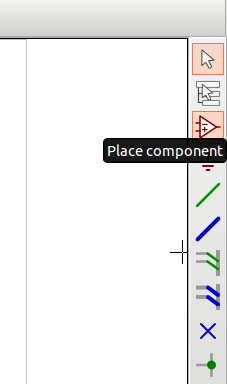
\includegraphics[width=\linewidth]{figures/rc_component.png}
    \caption{Place Component Icon}
    \label{rc_component}
\end{figure}

\pagebreak

After all the required components of the simple RC circuit are placed, wiring is done using the {\tt Place Wire} option as shown in the \figref{rc_wire} 

\begin{figure}[!htp]
    \centering
    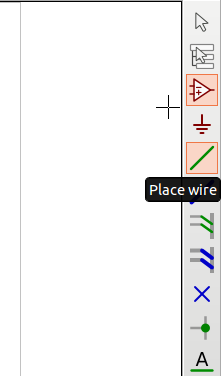
\includegraphics[width=\tnfig]{figures/rc_wire.png}
    %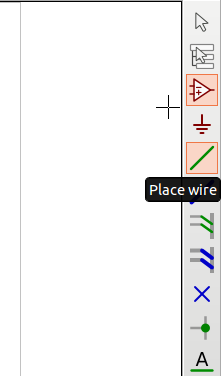
\includegraphics[width=\linewidth]{figures/rc_wire.png}
    \caption{Place Wire Icon}
    \label{rc_wire}
\end{figure}

Next step is {\tt ERC (Electric Rules Check)}. \figref{erc1} shows the icon for {\tt ERC}.

\begin{figure}[!htp]
    \centering
    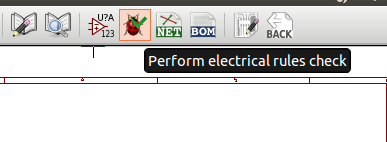
\includegraphics[width=\lgfig]{figures/erc1.png}
    %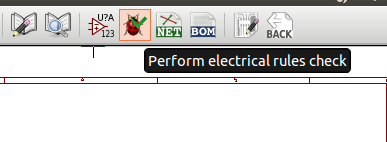
\includegraphics[width=\linewidth]{figures/erc1.png}
    \caption{Electric Rules Check Icon}
    \label{erc1}
\end{figure}

\figref{rc_complete1} shows the RC circuit after connecting the components by wire.

\begin{figure}[!htp]
    \centering
    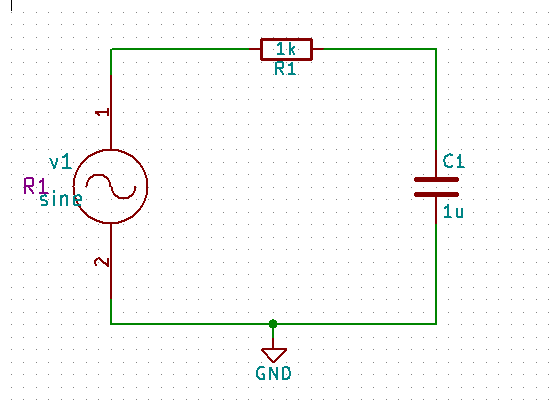
\includegraphics[width=\lgfig]{figures/rc_complete1.png}
    \caption{RC circuit}
    \label{rc_complete1}
\end{figure}

\pagebreak

After clicking the {\tt ERC} icon a window opens up. Click the {\tt Run} button to run rules check. The errors are listed in as shown in \figref{erc2}. This error is handled by adding {\tt Power Flag} as shown in \figref{rc_pwr}.

\begin{figure}[!htp]
    \centering
    \subfloat[ERC Run]{
        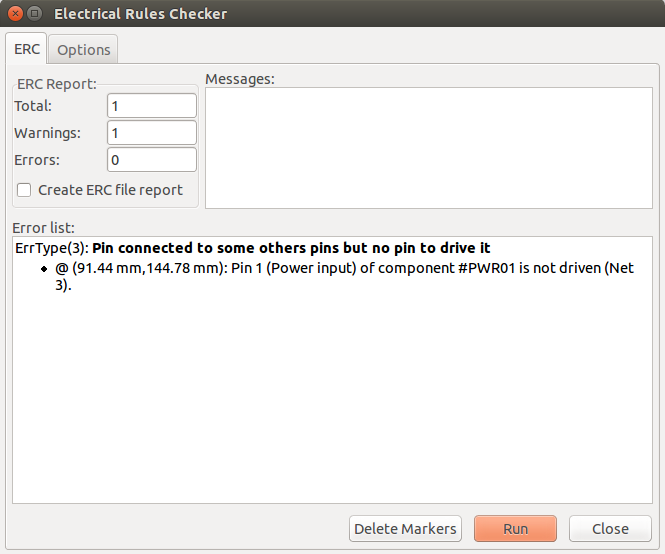
\includegraphics[width=\smfig]{figures/erc2.png}
    \label{erc2}} \hfill
    \subfloat[Power Flag]{
        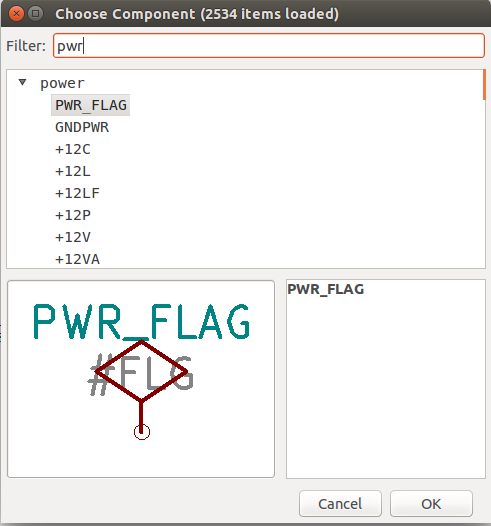
\includegraphics[width= 5cm, height=5cm]{figures/rc_pwr.png}
    \label{rc_pwr}}
    \caption{ERC check and POWER FLAG}
\end{figure}

After adding the {\tt Power Flag} the completed RC circuit is shown in \figref{rc_schematic} and the netlist is generated as shown in \figref{rc_netlist}.


\begin{figure}[!htp]
    \centering
    \subfloat[Schematic of RC circuit]{
        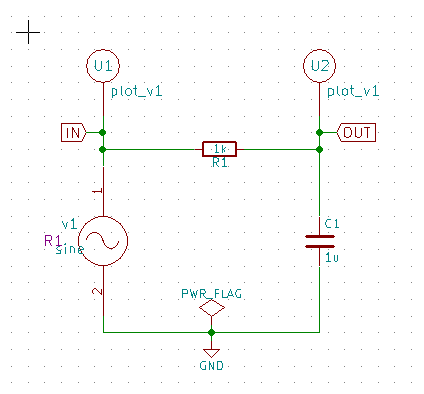
\includegraphics[width=\smfig]{figures/rc_schematic.png}
    \label{rc_schematic}} \hfill
    \subfloat[Generating KiCad Netlist of RC circuit]{
        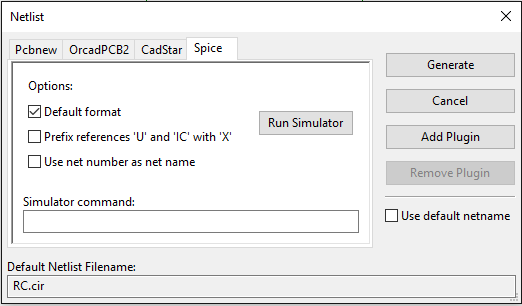
\includegraphics[width=\smfig]{figures/rc_netlistgeneration.png}
    \label{rc_netlist}}
    \caption{RC Schematic and Netlist Generation}
\end{figure}

\pagebreak
\item Convert KiCad to Ngspice:
To convert KiCad netlist of RC circuit to NgSpice compatible netlist click on KiCad to Ngspice icon as shown in \figref{rcki2ng}.

\begin{figure}[!htp]
\centering
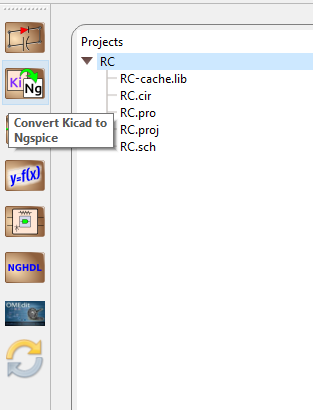
\includegraphics[width=\tnfig]{figures/rc_ki2ng.png}
\caption{Convert KiCad to Ngspice Icon}
\label{rcki2ng}
\end{figure}

Now you can enter the type of analysis and source details as shown in \figref{rc_analysistab} and \figref{rc_sourcedetailstab} respectively.

\begin{figure}[!htp]
    \centering
    \subfloat[RC Analysis]{
        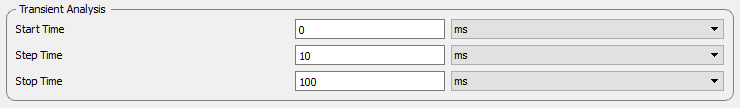
\includegraphics[width=\smfig]{figures/rc_analysistab.png}
    \label{rc_analysistab}} \hfill
    \subfloat[RC Source Details]{
        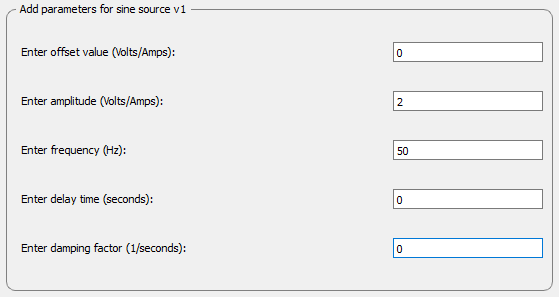
\includegraphics[width=\smfig]{figures/rc_sourcedetailstab.png}
    \label{rc_sourcedetailstab}}
    \caption{RC Analysis and Source Detail}
\end{figure}
The other tab will be empty as RC circuit do not use any Ngspice model, device library and subcircuit.

After entering the value, press the convert button. It will convert the netlist into Ngspice compatible netlist.

\pagebreak

\item Simulation:
To run Ngspice simulation click the simulation icon in the tool bar as shown in the \figref{rcplot}.
\begin{figure}[!htp]
\centering
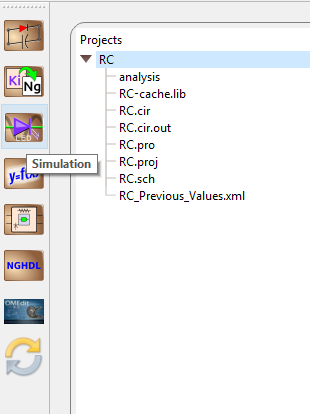
\includegraphics[width=\tnfig]{figures/rc_plot.png}
\caption{Simulation Icon}
\label{rcplot}
\end{figure}

In eSim, there are two types of plot. First is normal Ngspice plot and second is interactive python plot as shown in \figref{rc_ngspiceplot} and \figref{rc_pythonplot} respectively.

\begin{figure}[!htp]
    \centering
    \subfloat[Ngspice Plot of RC]{
        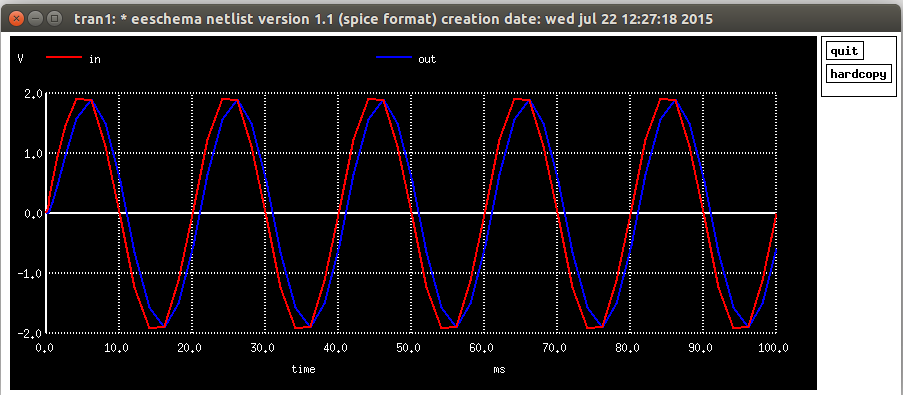
\includegraphics[width=\lgfig]{figures/rc_ngspiceplot.png}
    \label{rc_ngspiceplot}}  \hfill
    \subfloat[Python Plot of RC]{
        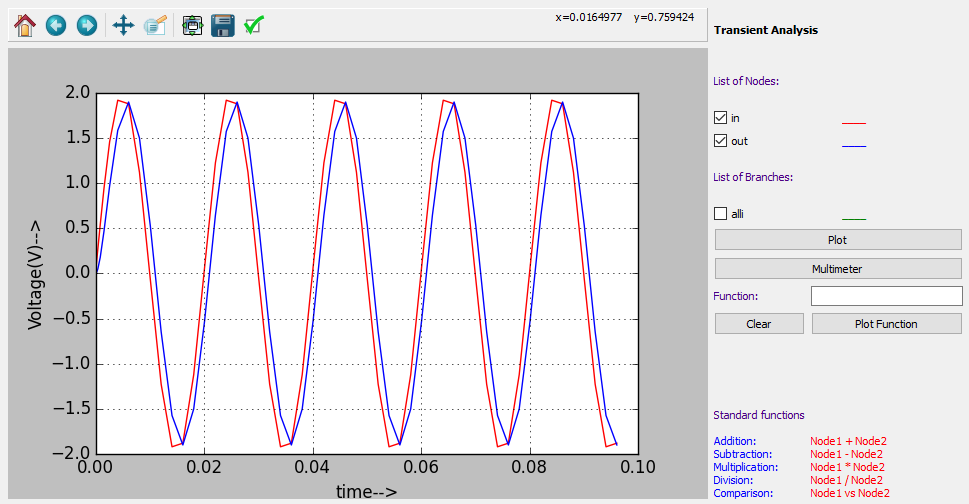
\includegraphics[width=\lgfig]{figures/rc_pythonplot.png}
    \label{rc_pythonplot}}
    \caption{Ngspice and Interactive Python Plotting}
\end{figure}

In the interactive python plot you can select any node or branch to  plot voltage or current across it. Also it has the facility to plot basic functions across the node like addition, substraction, multiplication, division and v/s.  

\end{itemize}
%-----------------------Half Wave Rectifier---------------------------
\pagebreak

\subsection{Half Wave Rectifier}

\subsubsection{Problem Statement:} Plot the Input and Output Waveform of Half Wave Rectifier circuit where the input voltage (Vs) is 50Hz, 2V peak to peak. The value for Resistor (R) is 1k.

\subsubsection{Solution:}
The new project is created by clicking the {\tt New} icon on the menubar. The name of the project is given in the window shown in \figref{rc1}.

\begin{itemize}
\item Creating Schematic:
To create the schematic, click the very first icon of the left toolbar as shown in the \figref{rc2}. This will open KiCad Eeschema.\\

After the KiCad window is opened, to create a schematic we need to place the required components. \figref{rc_component} shows the icon on the 
right toolbar which opens the component library.\\

After all the required components of the simple Half Wave rectifier circuits are placed, wiring is done using the {\tt Place Wire} option as shown in the \figref{rc_wire}\\

Next step is {\tt ERC (Electric Rules Check)}. \figref{erc1} shows the icon for {\tt ERC}. After completing all the above steps the final Half Wave Rectifier schematic will look like \figref{hwr_schematic}.\\

\begin{figure}[!htp]
    \centering
    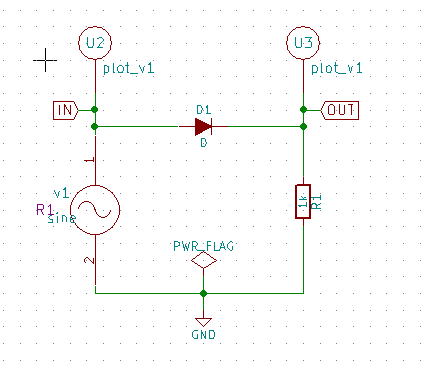
\includegraphics[width=\lgfig]{figures/hwr_schematic.png}
    \caption{Schematic of Half Wave Rectifier circuit}
    \label{hwr_schematic}
\end{figure}

\pagebreak

KiCad netlist is generated as shown in the \figref{hwr_netlistgeneration} \\

\begin{figure}[!htp]
    \centering
    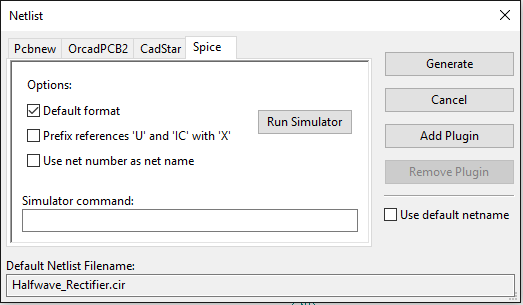
\includegraphics[width=\lgfig]{figures/hwr_netlistgeneration.png}
    \caption{Half Wave Rectifier circuit Netlist Generation}
    \label{hwr_netlistgeneration}
\end{figure}

\item Convert KiCad to Ngspice: After creating KiCad netlist, click on the {\tt KiCad-Ngspice converter} button. This will open converter window where you can enter details of Analysis, Source values and Device library.

\begin{figure}[!htp]
    \centering
    \subfloat[Half Wave Rectifier Analysis]{
        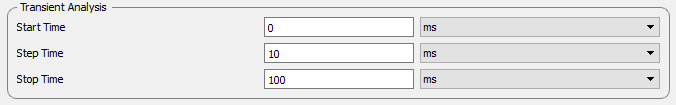
\includegraphics[width=\smfig]{figures/hwr_analysistab.png}
    \label{hwr_analysistab}} \hfill
    \subfloat[Half Wave Rectifier Source Details]{
        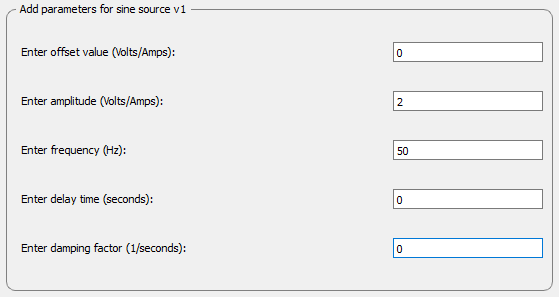
\includegraphics[width=\smfig]{figures/hwr_sourcedetailstab.png}
    \label{hwr_sourcedetailstab}} \hfill
    \subfloat[Half Wave Rectifier Device Modeling]{
        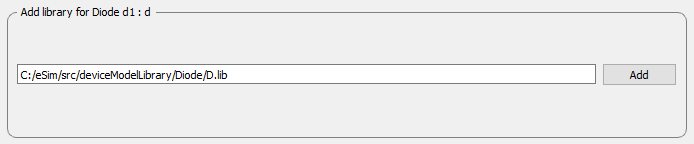
\includegraphics[width=\smfig]{figures/hwr_devicemodelingtab.png}
    \label{hwr_devicemodelingtab}}
    \caption{Analysis, Source and Device Tab}
\end{figure}

Under device library you can add the library for diode used in the circuit. If you do not add any library it will take default Ngspice model.


\item Simulation: Once the KiCad-Ngspice converter runs successfully, you can run simulation by clicking the simulation button in the toolbar.
\begin{figure}[!htp]
    \centering
    \subfloat[Ngspice Plot of Half Wave Rectifier]{
        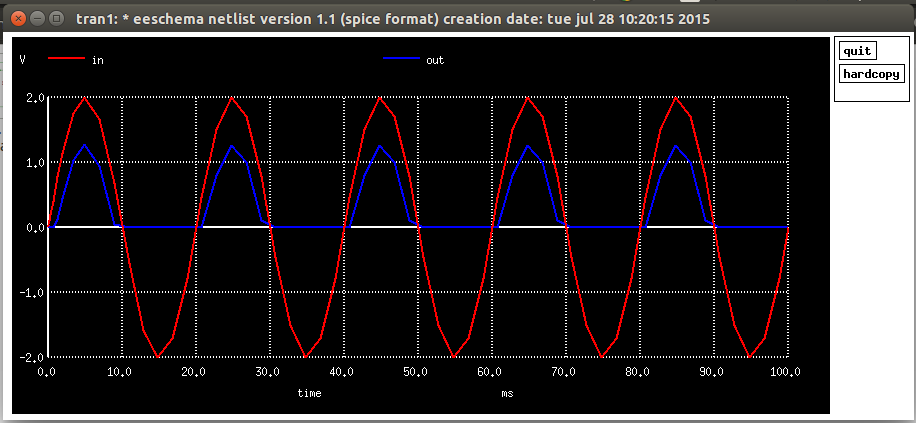
\includegraphics[width=\lgfig]{figures/hwr_ngspiceplot.png}
    \label{hwr_ngspiceplot}} \hfill
    \subfloat[Python Plot of Half Wave Rectifier]{
        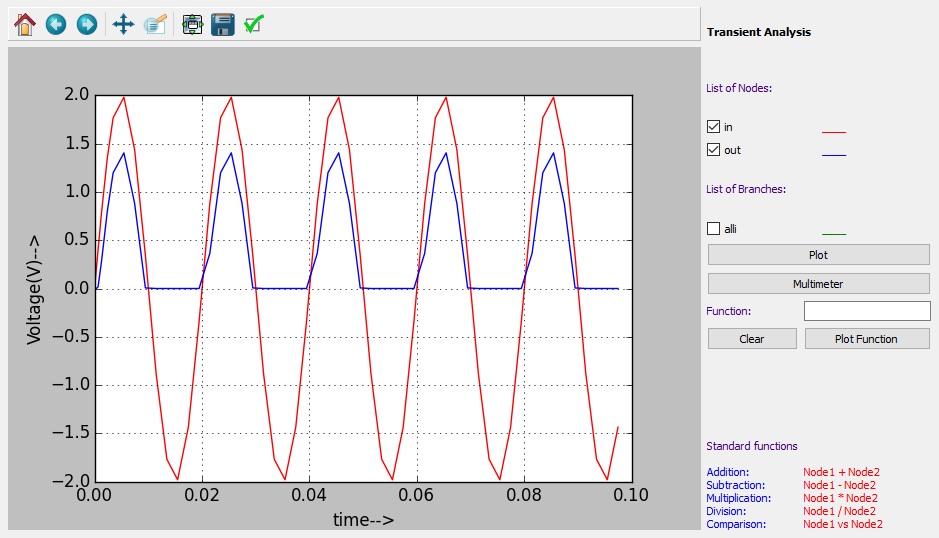
\includegraphics[width=\lgfig]{figures/hwr_pythonplot.png}
    \label{hwr_pythonplot}}
    \caption{Half Wave Rectifier Simulation Output}
\end{figure}


\end{itemize}

\pagebreak
%-------------- Precision rectifier--------------------------------------

%\pagebreak

%\subsection{Precision Rectifier}
%\subsubsection{Problem Statement:} Plot the input and output waveform of the Precision Rectifier circuit where input voltage (Vs) is $50Hz$ , $3V$ peak to peak.

%\subsubsection{Solution:}
%The new project is created by clicking the {\tt New} icon on the menubar. The name of the project is given as shown in the \figref{rc1}.

%\begin{itemize}
%\item Creating Schematic:
%To create the schematic, click the very first icon of the left toolbar as shown in the \figref{rc2}. This will open KiCad Eeschema.\\
%After the KiCad window is opened, to create a schematic we need to place the required components. \figref{rc_component} shows the icon on the right toolbar which opens the component library.\\
%After all the required components of the precision rectifier circuit are placed, wiring is done using the {\tt Place Wire} option as shown in the \figref{rc_wire}.\\
%Next step is {\tt ERC (Electric Rules Check)}. \figref{erc1} shows the icon for {\tt ERC}.
%The \figref{pr_schematic} shows the complete Precision Rectifier schematic after removing the errors.

%\begin{figure}[!htp]
%\centering
%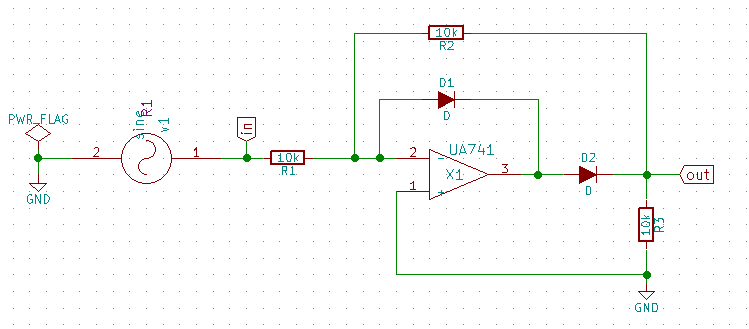
\includegraphics[width=\hgfig]{figures/pr_schematic.png}
%\caption{Schematic of Precision Rectifier circuit}
%\label{pr_schematic}
%\end{figure}

%The KiCad netlist is generated as shown in \figref{pr_netlistgeneration}.\\

%\begin{figure}[!htp]
%    \centering
%    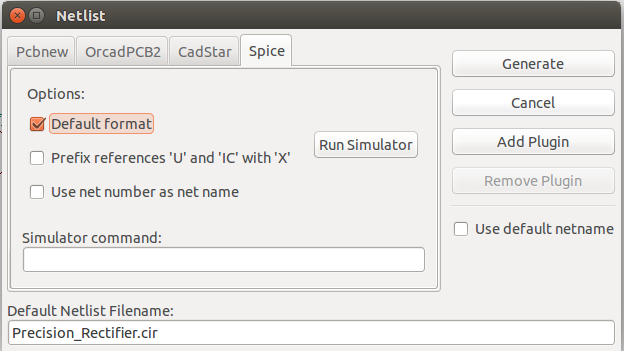
\includegraphics[width=\lgfig]{figures/pr_netlistgeneration.png}
%    \caption{Precision Rectifier circuit Netlist Generation}
%    \label{pr_netlistgeneration}
%\end{figure}

%\pagebreak

%\item Convert KiCad to Ngspice: After creating KiCad netlist, click on KiCad-Ngspice converter button.\\ 

%    This will open converter window where you can enter details of Analysis, Source values, Device library and Subcircuit.

%\begin{figure}[!htp]
%   \centering
%    \subfloat[Precision Rectifier Analysis]{
%        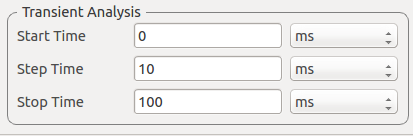
\includegraphics[width=\smfig]{figures/pr_analysistab.png}
%    \label{pr_analysistab}} \hfill
%    \subfloat[Precision Rectifier Source Details]{
%        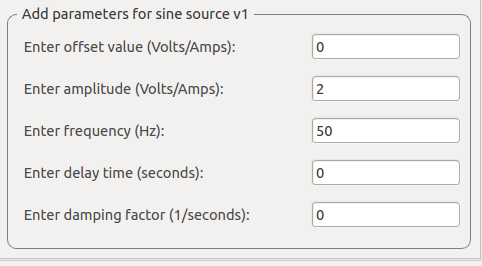
\includegraphics[width=\smfig]{figures/pr_sourcedetailstab.png}
%    \label{pr_sourcedetailstab}} \vfill
%    \subfloat[Precision Rectifier Device Modeling]{
%        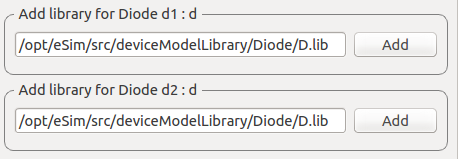
\includegraphics[width=\smfig]{figures/pr_devicemodelingtab.png}
%    \label{pr_devicemodelingtab}}\hfill
%    \subfloat[Precision Rectifier Subcircuit]{
%        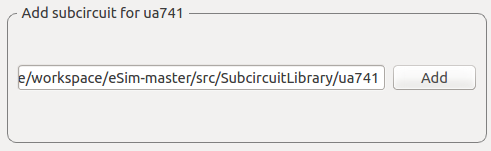
\includegraphics[width=\smfig]{figures/pr_subcircuitstab.png}
%    \label{pr_subcircuitstab}}
%    \caption{Analysis, Source, Device library and Subcircuit tab}
%\end{figure}

%Under device library you can add the library for the diode used in the circuit. If you do not add any library it will take default Ngspice 
%model for diode.\\

%Under subcircuit tab you have to add the subciruit used in your circuit. If you forget to add subcircuit it will throw an error.


%\pagebreak
%\item Simulation: Once the KiCad-Ngspice converter runs successfully, you can run the simulation by clicking the simulation button in the toolbar.
%\begin{figure}[!htp]
%    \centering
%    \subfloat[Ngspice Plot of Precision Rectifier]{
%        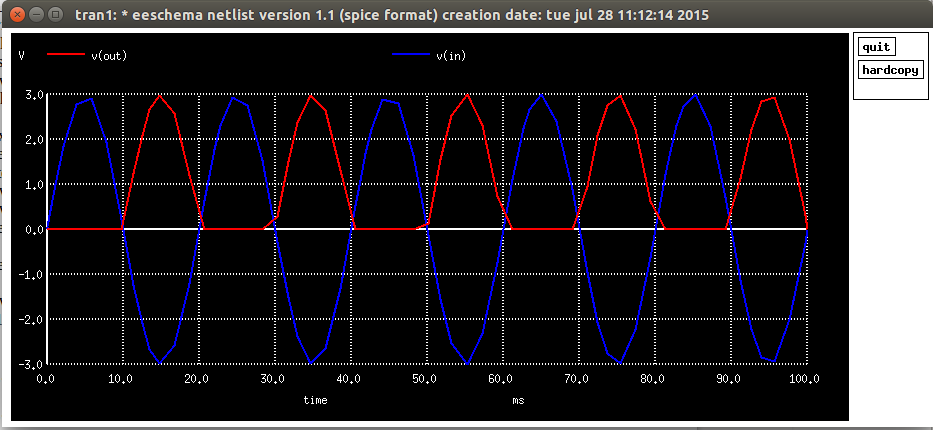
\includegraphics[width=\lgfig]{figures/pr_ngspiceplot.png}
%    \label{pr_ngspiceplot}} \hfill
%    \subfloat[Python Plot of Precision Rectifier]{
%        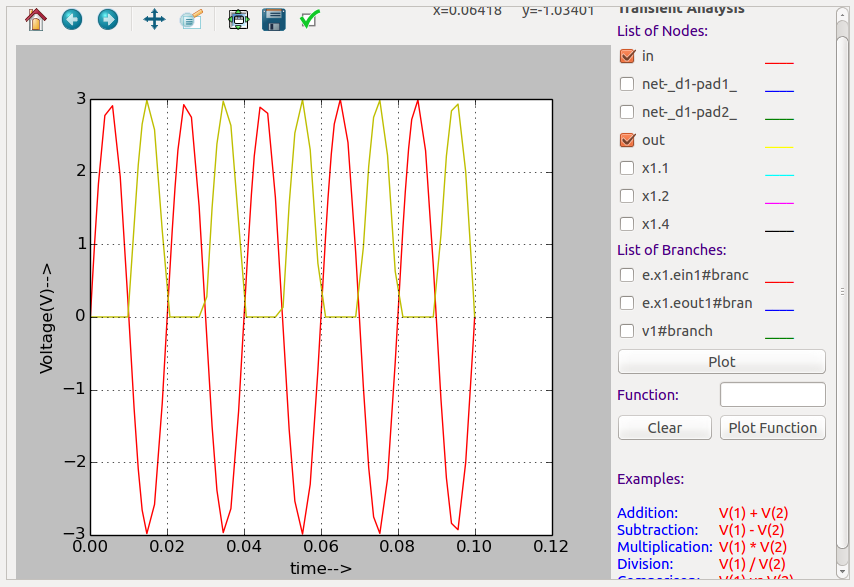
\includegraphics[width=\lgfig]{figures/pr_pythonplot.png}
%    \label{pr_pythonplot}}
%    \caption{Precision Rectifier Simulation Output}
%\end{figure}

%\end{itemize}

%-------------- Inverting Amplifier--------------------------------------

\pagebreak
\subsection{Inverting Amplifier}
\subsubsection{Problem Statement:}
Plot the Input and Output Waveform of Inverting Amplifier circuit where the input voltage (Vs) is $50Hz$, $2V$ peak to peak and gain is 2.
\subsubsection{Solution:}

\begin{itemize}
\item Creating Schematic:
To create the schematic, click the very first icon of the left toolbar as shown in the \figref{rc2}. This will open KiCad Eeschema.\\
After the KiCad window is opened, to create a schematic we need to place the required components. \figref{rc_component} shows the icon on the right toolbar which opens the component library.\\
After all the required components of the inverting amplifier circuit are placed, wiring is done using the {\tt Place Wire} option as shown in the \figref{rc_wire}.\\
Next step is {\tt ERC (Electric Rules Check)}. \figref{erc1} shows the icon for {\tt ERC}.

The \figref{ia_schematic} shows the complete Precision Rectifier schematic after removing the errors.

\begin{figure}[!htp]
    \centering
    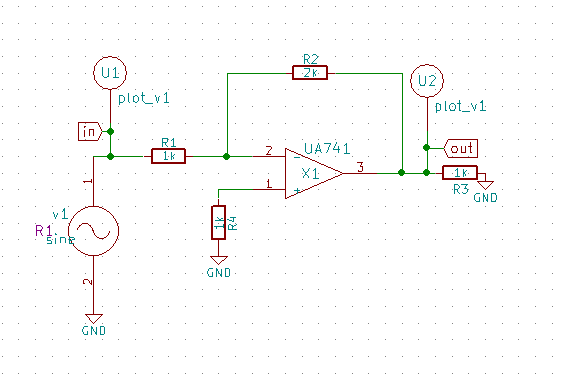
\includegraphics[width=\hgfig]{figures/ia_schematic.png}
    \caption{Schematic of Inverting Amplifier circuit}
    \label{ia_schematic}
\end{figure}

The KiCad netlist is generated as shown in \figref{ia_netlistgeneration}.\\
\begin{figure}[!htp]
    \centering
    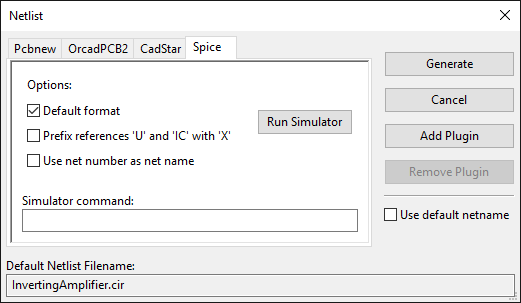
\includegraphics[width=\lgfig]{figures/ia_netlistgeneration.png}
    \caption{Inverting Amplifier circuit Netlist Generation}
    \label{ia_netlistgeneration}
\end{figure}


\item Convert KiCad to Ngspice:
After creating KiCad netlist, click on KiCad-Ngspice converter button.\\

This will open converter window where you can enter details of Analysis, Source values, Device library and Subcircuit.

Subcircuit of Op-Amp is shown in \figref{ia_sub}
    \begin{figure}[!htp]
        \centering
        \subfloat[Inverting Amplifier Analysis]{
            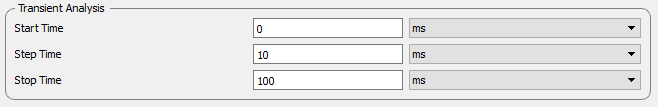
\includegraphics[width=\smfig]{figures/ia_analysistab.png}
        \label{ia_analysistab}} \hfill
        \subfloat[Inverting Amplifier Source Details]{
            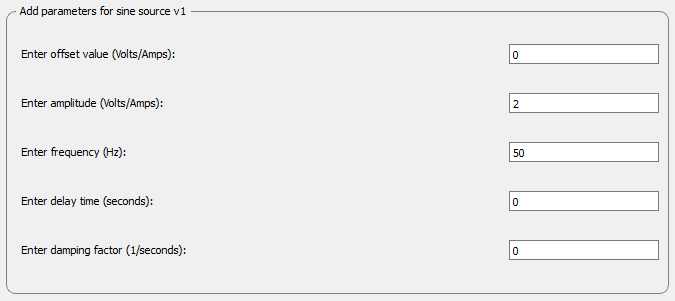
\includegraphics[width=\smfig]{figures/ia_sourcedetailstab.png}
        \label{ia_sourcedetailstab}} \vfill
        \subfloat[Inverting Amplifier Subcircuit]{
            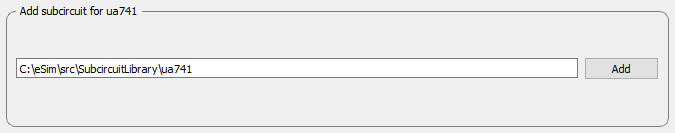
\includegraphics[width=\smfig]{figures/ia_subcircuitstab.png}
        \label{ia_subcircuitstab}}\hfill
        \subfloat[Sub-Circuit of Op-Amp]{
            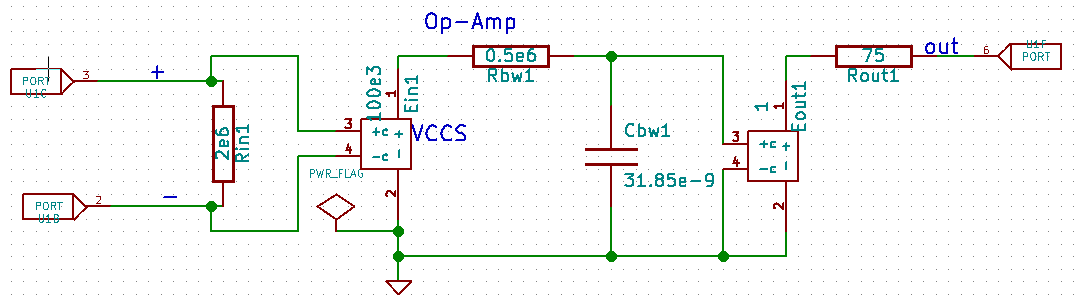
\includegraphics[width=\lgfig]{figures/ia_sub.png}
        \label{ia_sub}}
        \caption{Analysis, Source, and Subcircuit tab}
    \end{figure}

\pagebreak
Under subcircuit tab you have to add the subciruit used in your circuit. If you forget to add subcircuit, it will throw an error.\\


\item Simulation: Once the KiCad-Ngspice converter runs successfully, you can run simulation by clicking the simulation button in the toolbar.
\begin{figure}
    \centering
    \subfloat[Inverting Amplifier Ngspice Plot]{
        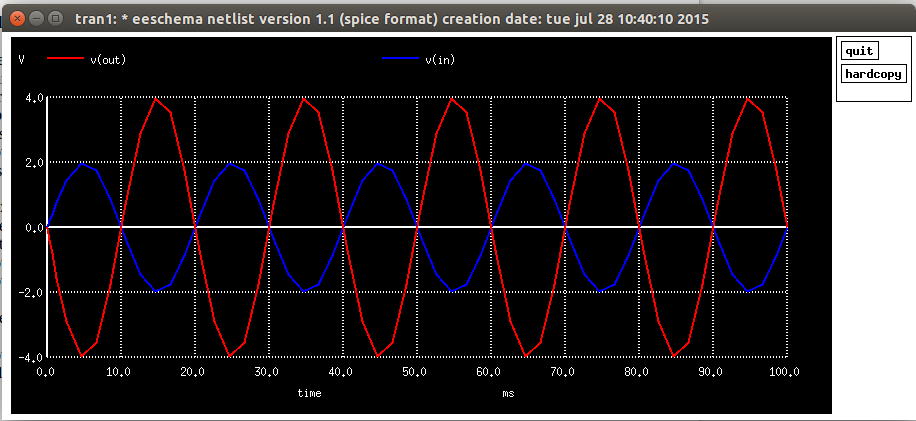
\includegraphics[width=\lgfig]{figures/ia_ngspiceplot.png}
    \label{ia_ngspiceplot}}\vfill
    \subfloat[Inverting Amplifier Python Plot]{
        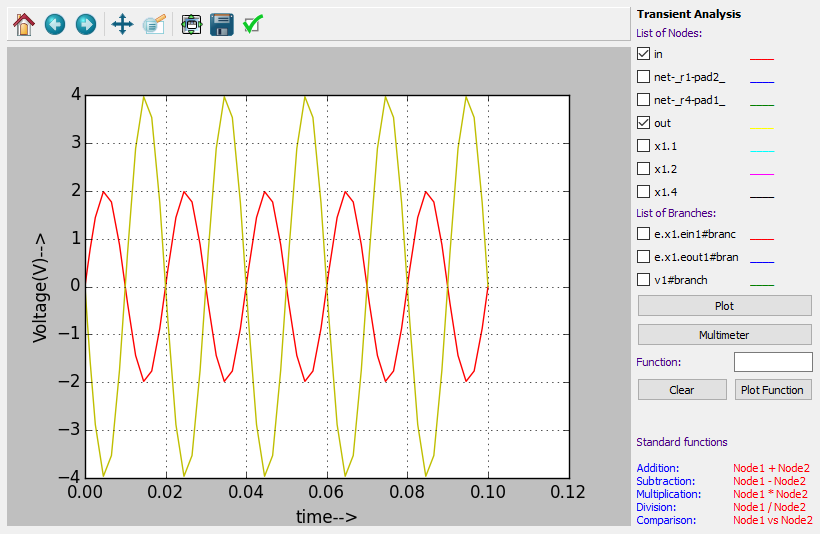
\includegraphics[width=\lgfig]{figures/ia_pythonplot.png}
    \label{ia_pythonplot}}
    \caption{Inverting Amplifier Simulation Output}
\end{figure}



\end{itemize}

%-------------------------Half Adder------------------------------------------

\pagebreak

\subsection{Half Adder}

\subsubsection{Problem Statement:}  Plot the Input and Output Waveform of Half Adder circuit.

\subsubsection{Solution:}

\begin{itemize}

\item Creating Schematic:  To create the schematic, click the very first icon of the left toolbar as shown in the \figref{rc2}. This will open KiCad Eeschema.\\
After the KiCad window is opened, to create a schematic we need to place the required components. \figref{rc_component} shows the icon on the right toolbar which opens the component library.\\
After all the required components of the Half Adder circuit are placed, wiring is done using the {\tt Place Wire} option as shown in the \figref{rc_wire}.\\
Next step is {\tt ERC (Electric Rules Check)}. \figref{erc1} shows the icon for {\tt ERC}.

The \figref{ha_schematic} shows the complete Half Adder schematic after removing the errors.
\begin{figure}[!htp]
    \centering
    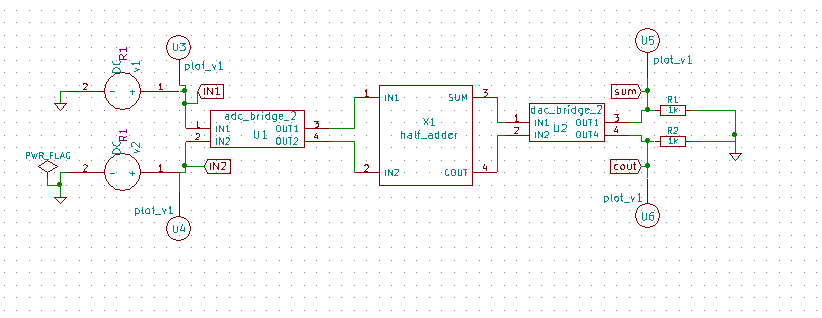
\includegraphics[width=\hgfig]{figures/ha_schematic.png}
    \caption{Schematic of Half Adder circuit}
    \label{ha_schematic}
\end{figure}

The KiCad netlist is generated as shown in \figref{ha_netlistgeneration}.\\
\begin{figure}[!htp]
    \centering
    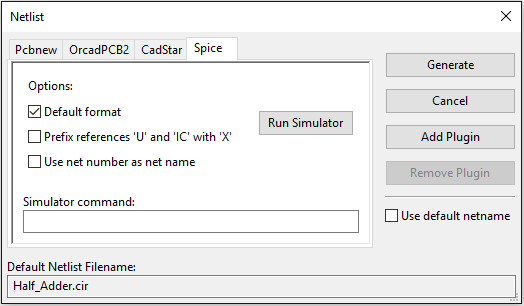
\includegraphics[width=\lgfig]{figures/ha_netlistgeneration.png}
    \caption{Half Adder circuit Netlist Generation}
    \label{ha_netlistgeneration}
\end{figure}

\pagebreak

\item Convert KiCad to Ngspice:
After creating KiCad netlist click on KiCad-Ngspice converter button.\\

This will open converter window where you can enter details of Analysis, Source values, Ngspice model and Subcircuit.

\begin{figure}[!htp]
    \centering
    \subfloat[Half Adder Analysis]{
        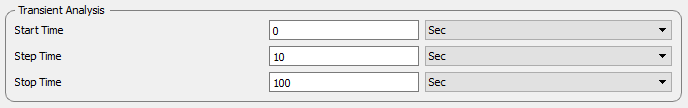
\includegraphics[width=\smfig]{figures/ha_analysistab.png}
    \label{ha_analysistab}} \hfill
    \subfloat[Half Adder Source Details]{
        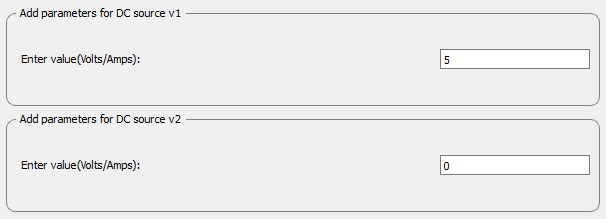
\includegraphics[width=\smfig]{figures/ha_sourcedetailstab.png}
    \label{ha_sourcedetailstab}} \vfill
    \subfloat[Half Adder Ngspice Model]{
        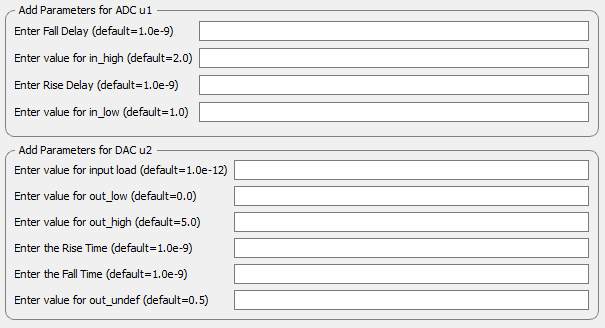
\includegraphics[width=\smfig]{figures/ha_ngspicemodeltab.png}
    \label{ha_ngspicemodeltab}} \hfill
    \subfloat[Half Adder Subcircuit Model]{
        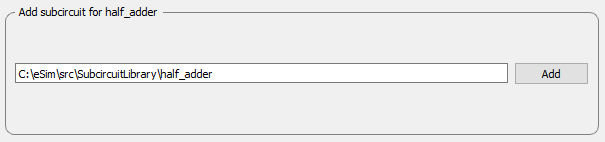
\includegraphics[width=\smfig]{figures/ha_subcircuitstab.png}
    \label{ha_subcircuitstab}}
    \caption{Analysis, Source, Ngspice Model and Subcircuit tab}
\end{figure}

Subcircuit of Half Adder in \figref{ha_sub}
\begin{figure}[!htp]
    \centering
    \includegraphics[width=\lgfig]{figures/ha_sub.png}
    \caption{Half Adder Subcircuit}
    \label{ha_sub}
\end{figure}

\pagebreak

\item Simulation: Once the KiCad-Ngspice converter runs successfully, you can run simulation by clicking the simulation button in the toolbar.
    \begin{figure}[!htp]
    \centering
    \subfloat[Half Adder Ngspice Plot]{
        \includegraphics[width=\lgfig]{figures/ha_ngspiceplot.png}
    \label{ha_ngspiceplot}} \hfill
    \subfloat[Half Adder Python Plot]{
        \includegraphics[width=\lgfig]{figures/ha_pythonplot.png}
    \label{ha_pythonplot}}
    \caption{Half Adder Simulation Output}
\end{figure}

\end{itemize}


%-------------------------Full Wave Rectifier using SCR------------------------------------------


\pagebreak

\subsection{Full Wave Rectifier using SCR}

\subsubsection{Problem Statement:}  Plot the Input and Output Waveform of Full Wave Rectifier using SCR.

\subsubsection{Solution:}

\begin{itemize}

\item Creating Schematic:  To create the schematic, click the very first icon of the left toolbar as shown in the \figref{rc2}. This will open KiCad Eeschema.\\
After the KiCad window is opened, to create a schematic we need to place the required components. \figref{rc_component} shows the icon on the right toolbar which opens the component library.\\
After all the required components of the Full Wave Rectifier using SCR circuit are placed, wiring is done using the {\tt Place Wire} option as shown in the \figref{rc_wire}.\\
Next step is {\tt ERC (Electric Rules Check)}. \figref{erc1} shows the icon for {\tt ERC}.

The \figref{fwrscr_schematic} shows the complete Rectifier circuit using SCR after removing the errors.
\begin{figure}[!htp]
    \centering
    \includegraphics[width=\hgfig]{figures/fwrscr_schematic.png}
    \caption{Schematic of Full Wave Rectifier using SCR}
    \label{fwrscr_schematic}
\end{figure}

The KiCad netlist is generated as shown in \figref{fwrscr_netlistgeneration}.\\
\begin{figure}[!htp]
    \centering
    \includegraphics[width=\lgfig]{figures/fwrscr_netlistgeneration.png}
    \caption{Full Wave Rectifier using SCR Netlist Generation}
    \label{fwrscr_netlistgeneration}
\end{figure}

\pagebreak

\item Convert KiCad to Ngspice:
After creating KiCad netlist click on KiCad-Ngspice converter button.\\

This will open converter window where you can enter details of Analysis, Source values, Ngspice model and Subcircuit.

\begin{figure}[!htp]
    \centering
    \subfloat[Full Wave Rectifier using SCR Analysis]{
        \includegraphics[width=\smfig]{figures/fwrscr_analysistab.png}
    \label{fwrscr_analysistab}} \hfill
    \subfloat[Full Wave Rectifier using SCR Source Details]{
        \includegraphics[width=\smfig]{figures/fwrscr_sourcedetailstab.png}
    \label{fwrscr_sourcedetailstab}} \vfill
    \subfloat[Full Wave Rectifier using SCR Subcircuit Model]{
        \includegraphics[width=\smfig]{figures/fwrscr_subcircuitstab.png}
    \label{fwrscr_subcircuitstab}}
    \caption{Analysis, Source and Subcircuit tab}
\end{figure}

Subcircuit of SCR in \figref{scr_sub}
\begin{figure}[!htp]
    \centering
    \includegraphics[width=\lgfig]{figures/scr_sub.png}
    \caption{SCR Subcircuit}
    \label{scr_sub}
\end{figure}

\pagebreak

\item Simulation: Once the KiCad-Ngspice converter runs successfully, you can run simulation by clicking the simulation button in the toolbar.
    \begin{figure}[!htp]
    \centering
    \subfloat[Full Wave Rectifier using SCR Ngspice Plot]{
        \includegraphics[width=\lgfig]{figures/fwrscr_ngspiceplot.png}
    \label{fwrscr_ngspiceplot}} \hfill
    \subfloat[Full Wave Rectifier using SCR Python Plot]{
        \includegraphics[width=\lgfig]{figures/fwrscr_pythonplot.png}
    \label{fwrscr_pythonplot}}
    \caption{Full Wave Rectifier using SCR Simulation Output}
\end{figure}

\end{itemize}


%-------------------------Oscillator------------------------------------------
\pagebreak

\subsection{Oscillator Circuit}

\subsubsection{Problem Statement:} Plot the Oscillation Waveforms for Phase Shift Oscillator circuit.

\subsubsection{Solution:}
The new project is created by clicking the {\tt New} icon on the menubar. The name of the project is given in the window shown in \figref{rc1}.

\begin{itemize}
\item Creating Schematic:
To create the schematic, click the very first icon of the left toolbar as shown in the \figref{rc2}. This will open KiCad Eeschema.\\

After the KiCad window is opened, to create a schematic we need to place the required components. \figref{rc_component} shows the icon on the 
right toolbar which opens the component library.\\

After all the required components of the Oscillator circuits are placed, wiring is done using the {\tt Place Wire} option as shown in the \figref{rc_wire}\\sss

Next step is {\tt ERC (Electric Rules Check)}. \figref{erc1} shows the icon for {\tt ERC}. After completing all the above steps the Oscillator schematic will look like \figref{osc_schematic}.\\

\begin{figure}[!htp]
    \centering
    \includegraphics[width=\lgfig]{figures/osc_schematic.png}
    \caption{Schematic of Phase Shift Oscillator circuit}
    \label{osc_schematic}
\end{figure}

\pagebreak

KiCad netlist is generated as shown in the \figref{osc_netlistgeneration} \\

\begin{figure}[!htp]
    \centering
    \includegraphics[width=\lgfig]{figures/osc_netlistgeneration.png}
    \caption{Phase Shift Oscillator circuit Netlist Generation}
    \label{osc_netlistgeneration}
\end{figure}

\item Convert KiCad to Ngspice: After creating KiCad netlist, click on the {\tt KiCad-Ngspice converter} button. This will open converter window where you can enter details of Analysis, Source values and Device library.

\begin{figure}[!htp]
    \centering
    \subfloat[Phase Shift Oscillator Analysis]{
        \includegraphics[width=\smfig]{figures/osc_analysistab.png}
    \label{osc_analysistab}} \hfill
    \subfloat[Phase Shift Oscillator Details]{
        \includegraphics[width=\smfig]{figures/osc_sourcedetailstab.png}
    \label{osc_sourcedetailstab}} \hfill
    \subfloat[Phase Shift Oscillator Device Modeling]{
        \includegraphics[width=\smfig]{figures/osc_devicemodelingtab.png}
    \label{osc_devicemodelingtab}}
    \caption{Analysis, Source and Device Tab}
\end{figure}

Under device library you can add the library for diode used in the circuit. If you do not add any library it will take default Ngspice model.


\item Simulation: Once the KiCad-Ngspice converter runs successfully, you can run simulation by clicking the simulation button in the toolbar.
\begin{figure}[!htp]
    \centering
    \subfloat[Ngspice Plot of Phase Shift Oscillator]{
        \includegraphics[width=\lgfig]{figures/osc_ngspiceplot.png}
    \label{osc_ngspiceplot}} \hfill
    \subfloat[Python Plot of Phase Shift Oscillator]{
        \includegraphics[width=\lgfig]{figures/osc_pythonplot.png}
    \label{osc_pythonplot}}
    \caption{Phase Shift Oscillator Simulation Output}
\end{figure}


\end{itemize}

%-------------------------BJT CB Characteristics------------------------------------------

\pagebreak

\subsection{Characteristics of BJT in Common Base Configuration}

\subsubsection{Problem Statement:} Plot Characteristics of BJT in Common Base Configuration.

\subsubsection{Solution:}
The new project is created by clicking the {\tt New} icon on the menubar. The name of the project is given in the window shown in \figref{rc1}.

\begin{itemize}
\item Creating Schematic:
To create the schematic, click the very first icon of the left toolbar as shown in the \figref{rc2}. This will open KiCad Eeschema.\\

After the KiCad window is opened, to create a schematic we need to place the required components. \figref{rc_component} shows the icon on the 
right toolbar which opens the component library.\\

After all the required components of the simple Half Wave rectifier circuits are placed, wiring is done using the {\tt Place Wire} option as shown in the \figref{rc_wire}\\

Next step is {\tt ERC (Electric Rules Check)}. \figref{erc1} shows the icon for {\tt ERC}. After completing all the above steps the BJT in CB Configuration schematic will look like \figref{cb_schematic}.\\

\begin{figure}[!htp]
    \centering
    \includegraphics[width=\lgfig]{figures/cb_schematic.png}
    \caption{Schematic of BJT in CB Configuration circuit}
    \label{cb_schematic}
\end{figure}

\pagebreak

KiCad netlist is generated as shown in the \figref{cb_netlistgeneration} \\

\begin{figure}[!htp]
    \centering
    \includegraphics[width=\lgfig]{figures/cb_netlistgeneration.png}
    \caption{BJT in CB Configuration circuit Netlist Generation}
    \label{cb_netlistgeneration}
\end{figure}

\item Convert KiCad to Ngspice: After creating KiCad netlist, click on the {\tt KiCad-Ngspice converter} button. This will open converter window where you can enter details of Analysis, Source values and Device library.

\begin{figure}[!htp]
    \centering
    \subfloat[BJT in CB Configuration Analysis]{
        \includegraphics[width=\smfig]{figures/cb_analysistab.png}
    \label{cb_analysistab}} \hfill
    \subfloat[BJT in CB Configuration Source Details]{
        \includegraphics[width=\smfig]{figures/cb_sourcedetailstab.png}
    \label{cb_sourcedetailstab}} \hfill
    \subfloat[BJT in CB Configuration Device Modeling]{
        \includegraphics[width=\smfig]{figures/cb_devicemodelingtab.png}
    \label{cb_devicemodelingtab}}
    \caption{Analysis, Source and Device Tab}
\end{figure}

Under device library you can add the library for diode used in the circuit. If you do not add any library it will take default Ngspice model.


\item Simulation: Once the KiCad-Ngspice converter runs successfully, you can run simulation by clicking the simulation button in the toolbar.
\begin{figure}[!htp]
    \centering
    \subfloat[Ngspice Plot of BJT in CB Configuration]{
        \includegraphics[width=\lgfig]{figures/cb_ngspiceplot.png}
    \label{cb_ngspiceplot}} \hfill
    \subfloat[Python Plot of BJT in CB Configuration]{
        \includegraphics[width=\lgfig]{figures/cb_pythonplot.png}
    \label{cb_pythonplot}}
    \caption{BJT in CB Configuration Simulation Output}
\end{figure}


\end{itemize}
